%% paper.tex -- ANN-based classification of DASS-42 severity levels with SHAP
%% Template: IEEEtran (bare_conf_compsoc), 4 pages.
%% Figures expected in ./figures/ (fig3_group_shares, fig6_beeswarm_D), as saved by the notebook.
%% Placeholders to fill are marked with \todo{...}.

\documentclass[conference,compsoc]{IEEEtran}

\ifCLASSOPTIONcompsoc
  \usepackage[nocompress]{cite}
\else
  \usepackage{cite}
\fi

\usepackage{graphicx}
\usepackage{amsmath}
\usepackage{url}
\usepackage{xcolor}

% visible placeholder for data still to be filled in
\newcommand{\todo}[1]{\textcolor{red}{[#1]}}

\hyphenation{op-tical net-works semi-conduc-tor}

\begin{document}

\title{ANN-Based Classification of Depression, Anxiety and Stress\\
from the DASS-42: Comparison with Classical Methods\\
and SHAP Interpretability}

\author{\IEEEauthorblockN{Mirko de Cillis}
\IEEEauthorblockA{Digital Transformation Management, University of Bologna\\
Machine Learning and Data Mining, A.Y.\ 2025/26\\
Email: decillis.web@gmail.com}}

\maketitle

\begin{abstract}
Questionnaire-based screening with the DASS-42 is widely used, and classical machine learning models recover its severity classes with high accuracy.
We study a multi-output artificial neural network (ANN) that predicts the five severity levels of depression, anxiety and stress at once from 34,583 validated online responses, and compare it with the baselines (RF, DT, NB, KNN, SVM) reported in a recent reference study.
A second experiment adds personality and demographic variables to test whether they carry information beyond the 42 items.
On a held-out test set of 12,105 respondents the ANN reaches 98.6\%, 100\% and 99.7\% accuracy on depression, anxiety and stress using the items alone, on par with the best baseline (SVM); all errors fall between adjacent severity levels.
Because the labels are a deterministic function of the items, this is a recovery of the scoring rule, not a diagnosis.
SHAP analysis shows that the network relies mostly on the items of the scale being predicted, nearly ignores personality items, and attributes the largest non-item weight to religion, which must be read as model reliance on a strongly imbalanced variable, not as a causal effect.
\end{abstract}

\section{Introduction}
Depression, anxiety and stress are among the most common mental health problems, and brief self-report instruments are a standard first screening tool.
The Depression Anxiety Stress Scales (DASS-42)~\cite{lovibond} contain 42 items rated from 0 to 3, 14 for each subscale; the sum of each subscale is mapped by fixed thresholds to five severity levels (normal, mild, moderate, severe, extremely severe).
A public dataset of about 40,000 online responses~\cite{kaggle} has become a common benchmark.
ShamsEldin et al.~\cite{shams} compared decision tree (DT), random forest (RF), naive Bayes (NB), k-nearest neighbours (KNN) and support vector machine (SVM) classifiers on it and found SVM the best, with 99.3\%, 98.9\% and 98.8\% accuracy on depression, anxiety and stress; they left deep learning as future work.
Srinath et al.~\cite{srinath} report a similar level (about 98\%) with logistic regression.

A property of this benchmark shapes the whole study: the severity labels are computed from the same 42 items given as input.
The task is therefore not to diagnose, but to recover a known additive scoring rule, and very high accuracy is expected.
We take this at face value and ask three narrower questions.
\textbf{Q1:} can a single multi-output ANN recover the three labels as well as the classical baselines?
\textbf{Q2:} do the personality (TIPI~\cite{tipi}) and demographic variables of the dataset add anything beyond the items?
\textbf{Q3:} which inputs does the trained network actually rely on, and does it behave as the scoring rule would predict?

Tree-based and kernel methods usually remain competitive on low-dimensional tabular data~\cite{gri}, so we do not expect the ANN to be better.
It is chosen as a deliberate empirical comparison, and because a shared trunk with one head per scale can exploit the correlation between the three scales.
The contributions are: (i) a multi-head ANN with class-weighted loss, evaluated with 5-fold cross-validation and a held-out test set on cleaned data; (ii) a controlled comparison between items only (Experiment A) and items plus TIPI and demographics (Experiment B); (iii) a SHAP~\cite{shap} analysis aggregated per original variable and per variable group, with additivity and stability checks.

\textbf{Group organization.}
The project was carried out individually (the course allows groups of at most two). The author designed and implemented the whole pipeline (data cleaning and labelling, ANN training and evaluation, SHAP analysis, figures) in a Google Colab notebook, and wrote this paper.
Notebook, paper and slides are available at \todo{GitHub repository URL}.

\section{Proposed Method}
\subsection{Data and preprocessing}
We use the public DASS-42 dataset~\cite{kaggle}: 39,775 responses, 172 columns, collected in 2017--2019.
Item answers, coded 1--4 in the file, were shifted to 0--3 as in the DASS manual.
We dropped item-position and item-timing columns, survey-level timing and technical fields, and variables unrelated to the construct (native language, handedness, voting, family size, country, major).
Following~\cite{shams}, responses where any of the three non-existent words of the validity checklist was ticked were treated as inattentive and removed: 5,192 rows (13.1\%), leaving 34,583.
Out-of-range values were repaired: ages given as birth years were converted using 2018 as reference year and three-digit typos corrected; invalid gender, religion and orientation were set to ``Other'', invalid marital status to ``never married'', invalid education or urbanicity to the most frequent valid value, invalid TIPI answers to the neutral value 4.
Categories under 1\% of the rows (three religions, three races) were merged into ``Other'', and the five nominal variables (gender, religion, orientation, marital status, race) were one-hot encoded.
The result has 79 features: 42 items, 10 TIPI items, age, education, urbanicity and the dummy variables.

\subsection{Labels and class imbalance}
For each respondent, the subscale scores are the sums of its 14 items (item assignment from the DASS handbook) and are mapped to five levels with the standard thresholds~\cite{lovibond}; for depression: 0--9 normal, 10--13 mild, 14--20 moderate, 21--27 severe, 28+ extremely severe.
The scores are kept outside the feature matrix, so there is no target leakage beyond the one inherent to the labelling rule.
Classes are imbalanced: extremely severe is the largest class for depression and anxiety (33.5\% and 34.8\%), normal for stress (29.9\%), and mild is the smallest (7--13\%).
Imbalance is handled with class weights in the loss (``balanced'' weights computed on the training set only), without resampling.

\subsection{Model}
The classifier is a feed-forward network in PyTorch~\cite{torch}.
A shared trunk of two fully connected layers (64 and 32 units, ReLU, dropout 0.2 after the first) feeds three independent linear heads, one per scale, each producing five logits.
The model has 5,327 parameters in Experiment A (42 inputs) and 7,695 in Experiment B (79 inputs).
The training loss is the sum of the three class-weighted cross-entropies,
\begin{equation}
\mathcal{L}=\sum_{s\in\{D,A,S\}}\mathrm{CE}_{w^{(s)}}\!\left(z^{(s)},y^{(s)}\right),
\end{equation}
where $z^{(s)}$ are the logits and $w^{(s)}$ the class weights of scale $s$.
We use Adam~\cite{adam} and early stopping on the validation loss, restoring the best weights.
Experiment A uses the 42 items only; Experiment B uses all 79 features.
Baselines (RF, DT, NB, KNN, SVM) were \emph{not} recomputed: we report the figures published in~\cite{shams}, which used a different preprocessing and a 70/30 split, so the comparison is indicative, not strictly like-for-like.

\subsection{Evaluation protocol}
The data are split 65/35 with stratification on the combination of the three labels: 22,478 training and 12,105 test respondents.
Features are standardized with a scaler fitted on training data only (within each fold in cross-validation).
Five-fold stratified cross-validation on the training set (stratified on the anxiety label, since some label combinations have fewer than five respondents) gives mean and standard deviation of each metric.
The final model is trained once on the training set (seed 42), with 10\% of it held out for early stopping, and evaluated once on the test set.
Training settings (up to 200 epochs, learning rate $3\cdot10^{-3}$, batch size 512, patience 10, minimum improvement $10^{-3}$) were adjusted after a first exploratory run; reported scores are therefore not from a pre-fixed configuration.
Metrics are accuracy, macro-F1 and weighted-F1; the latter is the F1 average used in~\cite{shams} and is the one compared with the baselines.

\subsection{Interpretability with SHAP}
We explain each scale with SHAP DeepExplainer~\cite{shap}, wrapping each head as a separate model that outputs its five logits.
The background is 100 random scaled training rows and the explained set a random subsample of 3,000 test rows (seed 0); values are on the logit scale.
The importance of a variable $v$ on scale $s$ is
\begin{equation}
I_v^{(s)}=\operatorname*{mean}_{n,\,c}\Big|\sum_{j\in \mathrm{dum}(v)}\phi^{(s)}_{n,j,c}\Big|,
\end{equation}
where $\phi$ are the SHAP values for sample $n$ and class $c$, and the dummies of a nominal variable are summed \emph{before} taking the absolute value.
Importances are normalized to 100\% per scale, and also summed over four groups: items of the scale itself (``own''), items of the other scales, TIPI, and demographics.
Shares are compared only within the same experiment, and measure model reliance, not causal effect or variance explained.
Two checks were run for both experiments: additivity (logits equal baseline plus the sum of SHAP values, maximum error between $3\cdot10^{-5}$ and $7.5\cdot10^{-5}$) and stability (Spearman correlation between the rankings from the two halves of the subsample, 0.996--0.998).

\section{Results}
\subsection{Comparison with classical baselines}
With items only, cross-validated accuracy (mean $\pm$ std over five folds) is 99.57$\pm$0.56\% for depression, 99.99$\pm$0.02\% for anxiety and 99.72$\pm$0.29\% for stress; with all features it is 99.13$\pm$0.51\%, 99.75$\pm$0.22\% and 98.51$\pm$1.21\%.
Table~\ref{tab:baselines} reports the test results next to the published baselines.
The ANN of Experiment A is far above RF, DT, NB and KNN and on par with SVM: slightly lower on depression (98.62\% vs.\ 99.3\%) and higher on anxiety and stress.
These differences are at most one percentage point, come from a single run, and use different splits and preprocessing, so we do not claim an advantage over SVM.

\begin{table}[!t]
\centering
\caption{Test accuracy and weighted F1 (\%). Baselines are taken from Table~3 of~\cite{shams} (not recomputed; different pipeline and split). ANN: single run, 12,105 test respondents. Best of A and the baselines in bold.}
\label{tab:baselines}
\footnotesize
\setlength{\tabcolsep}{3.5pt}
\begin{tabular}{l cc cc cc}
\hline
 & \multicolumn{2}{c}{Depression} & \multicolumn{2}{c}{Anxiety} & \multicolumn{2}{c}{Stress}\\
Model & Acc & F1 & Acc & F1 & Acc & F1\\
\hline
RF  & 92.8 & 92.6 & 85.2 & 82.9 & 88.8 & 88.4\\
DT  & 79.3 & 79.4 & 73.7 & 73.7 & 74.7 & 74.9\\
NB  & 87.2 & 87.7 & 81.3 & 82.0 & 85.2 & 85.7\\
KNN & 86.9 & 86.2 & 79.3 & 76.5 & 84.7 & 84.4\\
SVM & \textbf{99.3} & \textbf{99.3} & 98.9 & 98.9 & 98.8 & 98.8\\
\hline
ANN (A) & 98.62 & 98.63 & \textbf{100.0} & \textbf{100.0} & \textbf{99.69} & \textbf{99.69}\\
ANN (B)$^\dagger$ & 99.46 & 99.46 & 99.88 & 99.88 & 99.58 & 99.58\\
\hline
\multicolumn{7}{l}{\scriptsize $^\dagger$ Items + TIPI + demographics; not comparable with the baselines.}
\end{tabular}
\end{table}

\subsection{Error structure and items vs.\ all features}
\begin{figure*}[!t]
\centering
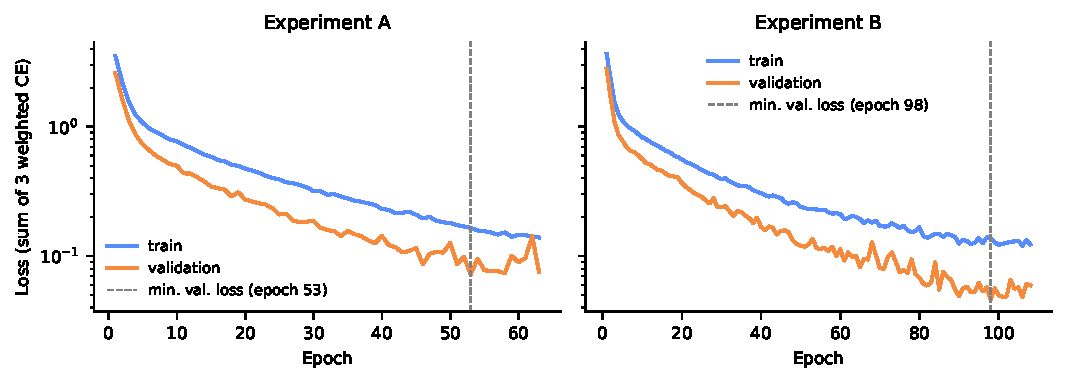
\includegraphics[width=0.92\textwidth]{figures/fig1_learning_curves}
\caption{Training and validation loss (sum of the three class-weighted cross-entropies) per epoch for the final models of Experiments A and B, on a logarithmic axis. The dashed line marks the epoch of minimum validation loss, where early stopping restores the weights.}
\label{fig:curves}
\end{figure*}

\begin{figure*}[!t]
\centering
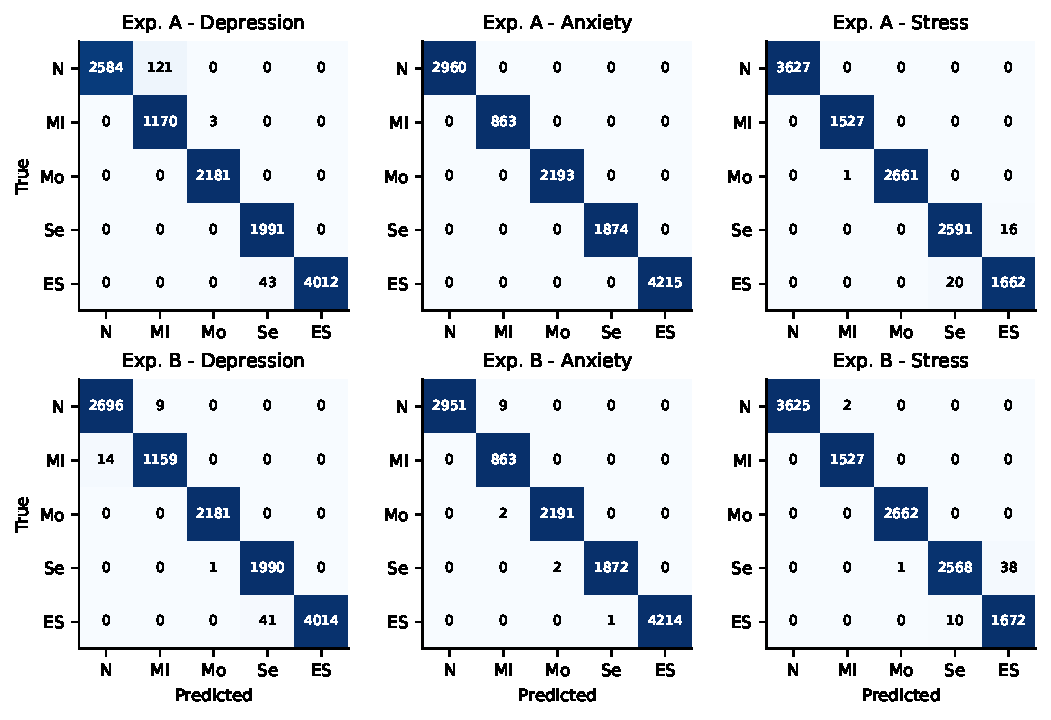
\includegraphics[width=0.92\textwidth]{figures/fig2_confusion}
\caption{Test-set confusion matrices (12,105 respondents): experiments in rows, scales in columns. Cells show counts, colour the row-normalised proportion. N, Mi, Mo, Se, ES: normal, mild, moderate, severe, extremely severe. Errors occur only between adjacent classes.}
\label{fig:conf}
\end{figure*}

Every misclassification occurs between adjacent severity levels (Fig.~\ref{fig:conf}), next to the score thresholds that define the labels.
With items only, depression has 121 normal$\to$mild, 43 extremely severe$\to$severe and 3 mild$\to$moderate errors (167 of 12,105), anxiety has none, and stress has 37 (16 severe$\to$extremely severe, 20 the reverse, 1 moderate$\to$mild).
With all features the errors are 65 on depression, 14 on anxiety and 51 on stress.
Adding TIPI and demographics gives no consistent gain: Experiment B is better on depression on the test set (99.46\% vs.\ 98.62\%) but worse in cross-validation (99.13\% vs.\ 99.57\%), and Experiment A is better on anxiety and stress on both.
With a single test run and differences below one point, we conclude only that the extra variables do not help.
Early stopping ended after 63 epochs (A) and 108 (B), including the 10 of patience; Fig.~\ref{fig:curves} shows the loss curves and the epoch of minimum validation loss.

\subsection{What the network relies on}
\begin{figure}[!t]
\centering
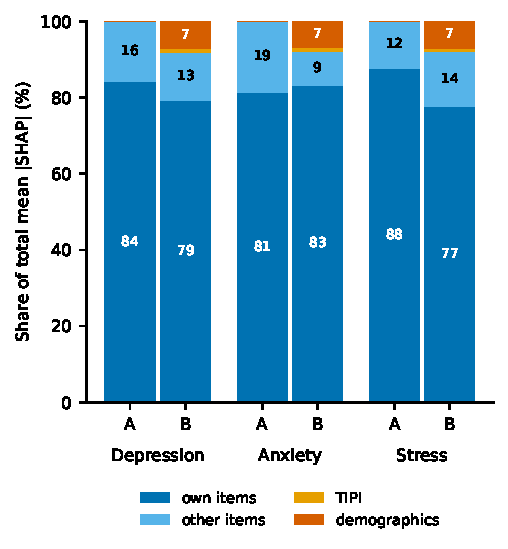
\includegraphics[width=0.85\columnwidth]{figures/fig3_group_shares}
\caption{Share of total mean $|$SHAP$|$ by variable group (own-scale items, other-scale items, TIPI, demographics) for each scale, Experiment A vs.\ B. Own-scale items dominate in both; in B, demographics carry about 7\% and TIPI about 1\%.}
\label{fig:groups}
\end{figure}

Fig.~\ref{fig:groups} shows the group shares.
In A, own-scale items carry 84.1\%, 81.2\% and 87.6\% of the importance (depression, anxiety, stress), and the remaining 12--19\% goes to items of the other scales, which are redundant for the label; this is consistent with the network exploiting the correlation among subscales rather than needing it.
In B, own items carry 79.1\%, 83.2\% and 77.5\%, other-scale items 9--14\%, demographics about 7\% and TIPI about 1\%.
Per variable, an own item weighs 5.5--6.0\%, a demographic variable about 0.9\%, an other-scale item 0.3--0.5\% and a TIPI item about 0.1\%.
TIPI variables never reach the top five non-own variables of any scale.
Fig.~\ref{fig:top15} ranks the 15 most important variables per scale in Experiment B: own-scale items dominate the ranking, and religion is the leading non-own variable.

\begin{figure*}[!t]
\centering
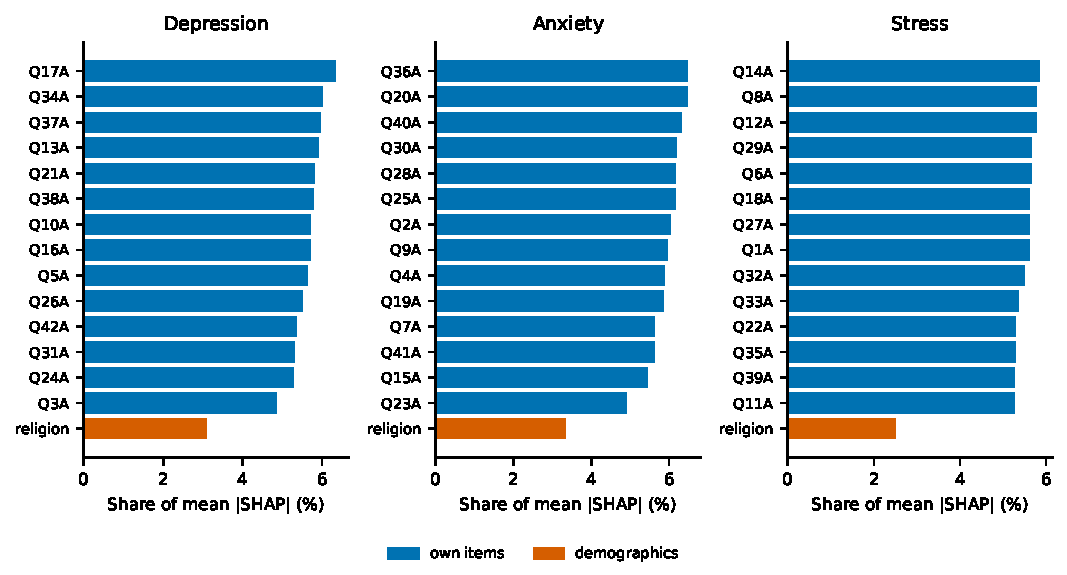
\includegraphics[width=0.92\textwidth]{figures/fig4_top15_B}
\caption{The 15 most important variables per scale in Experiment B, ranked by share of mean $|$SHAP$|$, with dummies of nominal variables aggregated per original variable. Bars are coloured by variable group; each panel has its own x-axis.}
\label{fig:top15}
\end{figure*}

\begin{figure}[!t]
\centering
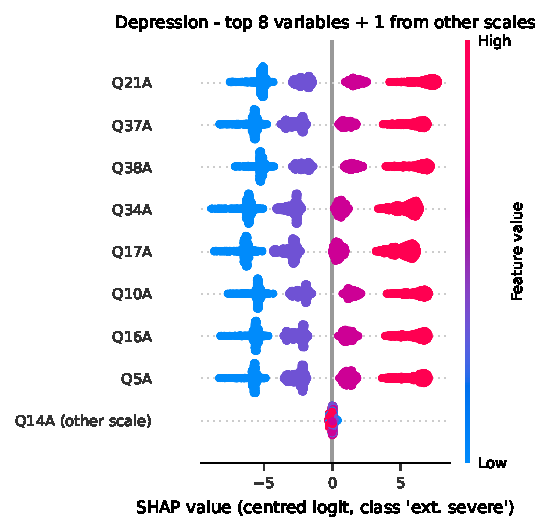
\includegraphics[width=0.9\columnwidth]{figures/fig6_beeswarm_D}
\caption{SHAP beeswarm for the depression head of Experiment B, class extremely severe, 3,000 test respondents. Each dot is a respondent coloured by feature value (grey: nominal). Depression items act monotonically: high answers raise the class logit, low answers lower it, as in an additive score.}
\label{fig:beeswarm}
\end{figure}

The beeswarm in Fig.~\ref{fig:beeswarm} shows that the depression items contribute with similar magnitude and in an ordered way, so the network has recovered the additive scoring rule.
Among the non-item variables of Experiment B, \emph{religion} is the most important on all scales (3.09\%, 3.34\%, 2.50\%), followed by race, marital status and gender (about 0.6--1.8\%).
Its per-class SHAP values on depression are lopsided: Muslim respondents (58\% of the sample, $n=1{,}739$ in the subsample) are pushed away from ``normal'' ($-3.57$) and towards severe ($+1.54$), while most other groups are pushed towards it (e.g.\ agnostic $+8.29$, atheist $+3.68$), and Catholic respondents are close to neutral ($+0.33$) (Fig.~\ref{fig:religion}).
Since attributions are measured against a Muslim-dominated background, they mainly reflect a Muslim vs.\ non-Muslim contrast; estimates for small groups are weak, and religion may act as a proxy for culture or country, which we removed.
It signals that the network exploits a demographic correlation present in this sample, not that religion influences mental health.

\begin{figure}[!t]
\centering
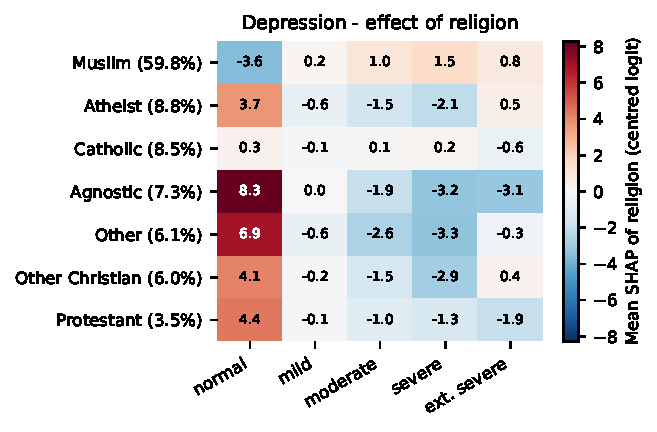
\includegraphics[width=0.95\columnwidth]{figures/fig5_religion_heatmap}
\caption{Mean SHAP of religion on each severity class of the depression head, Experiment B, for religions with at least 100 test samples (share of the subsample in brackets). Values are centred logits: red pushes towards the class, blue away. Measured against a Muslim-dominated background.}
\label{fig:religion}
\end{figure}

\section{Conclusions}
We trained a small multi-output ANN to classify the severity of depression, anxiety and stress from the DASS-42, and compared it with the classical baselines of a reference study.
On the test set it reaches 98.6\%, 100\% and 99.7\% accuracy with the items alone, comparable to the best classical model (SVM) and far above the other four; all errors are between adjacent levels.
Because the labels are computed from the items, these results measure how well the rule is recovered, and SHAP confirms it: depression items drive the depression output monotonically and with similar weight.
Adding personality and demographic variables brings no consistent gain, TIPI variables are practically ignored, and the weight given to demographics (about 7\%), religion above all, shows reliance on sample-specific correlations rather than clinical signal.

\textbf{Limitations.}
Baselines are copied from the reference paper and not recomputed; ANN results come from a single test run with training settings adjusted after a first run; SHAP shares describe model reliance, not causality, and use a 3,000-row subsample; the dataset is a self-selected online sample, with a strong imbalance on religion.
\textbf{Future work} includes recomputing the baselines on the same split, repeating the test over several seeds, testing robustness when items are missing (where the exact scoring rule cannot be applied), and a fairness analysis by gender and age.

\begin{thebibliography}{10}

\bibitem{shams}
T.~ShamsEldin \emph{et al.}, ``Artificial intelligence for predicting depression anxiety and stress using psychometric data,'' \emph{Sci. Rep.}, vol.~15, art.~37282, 2025, doi: 10.1038/s41598-025-21301-1.

\bibitem{lovibond}
S.~H. Lovibond and P.~F. Lovibond, \emph{Manual for the Depression Anxiety Stress Scales}, 2nd~ed. Sydney, Australia: Psychology Foundation of Australia, 1995.

\bibitem{kaggle}
``Depression Anxiety Stress Scales responses,'' Kaggle dataset (user \texttt{lucasgreenwell}). [Online]. Available: \url{https://www.kaggle.com/datasets/lucasgreenwell/depression-anxiety-stress-scales-responses}

\bibitem{tipi}
S.~D. Gosling, P.~J. Rentfrow, and W.~B. Swann~Jr., ``A very brief measure of the Big-Five personality domains,'' \emph{J. Res. Personality}, vol.~37, no.~6, pp.~504--528, 2003.

\bibitem{shap}
S.~M. Lundberg and S.-I. Lee, ``A unified approach to interpreting model predictions,'' in \emph{Proc. NeurIPS}, 2017, pp.~4765--4774.

\bibitem{gri}
L.~Grinsztajn, E.~Oyallon, and G.~Varoquaux, ``Why do tree-based models still outperform deep learning on typical tabular data?'' in \emph{Proc. NeurIPS Datasets and Benchmarks Track}, 2022.

\bibitem{torch}
A.~Paszke \emph{et al.}, ``PyTorch: An imperative style, high-performance deep learning library,'' in \emph{Proc. NeurIPS}, 2019, pp.~8024--8035.

\bibitem{adam}
D.~P. Kingma and J.~Ba, ``Adam: A method for stochastic optimization,'' in \emph{Proc. ICLR}, 2015.

\bibitem{srinath}
K.~Srinath \emph{et al.}, ``Prediction of depression, anxiety and stress levels using DASS-42,'' in \emph{Proc. Int. Conf. for Convergence in Technology}, IEEE, 2022.

\end{thebibliography}

\end{document}
